% !TeX document-id = {10b3ccb1-3544-4c78-abc6-ec60d098d2a0}
% !BIB TS-program = biber

\RequirePackage[l2tabu,orthodox]{nag}

% TODO: decide if one-sided/two-sided
%\documentclass[headsepline,footsepline,footinclude=false,fontsize=11pt,paper=a4,listof=totoc,bibliography=totoc,BCOR=12mm,DIV=12]{scrbook} % two-sided
\documentclass[headsepline,footsepline,footinclude=false,oneside,fontsize=11pt,paper=a4,listof=totoc,bibliography=totoc]{scrbook} % one-sided

% TODO: change citation style in settings
\PassOptionsToPackage{table,svgnames,dvipsnames}{xcolor}

\usepackage[utf8]{inputenc}
\usepackage[T1]{fontenc}
\usepackage[sc]{mathpazo}
\usepackage[ngerman,american]{babel}
\usepackage[autostyle]{csquotes}
\usepackage[%
  backend=biber,
  url=false,
  style=alphabetic,
  maxnames=4,
  minnames=3,
  maxbibnames=99,
  giveninits,
  uniquename=init]{biblatex} % TODO: adapt citation style
\usepackage{graphicx}
\usepackage{scrhack} % necessary for listings package
\usepackage{listings}
\usepackage{lstautogobble}
\usepackage{tikz}
\usepackage{pgfplots}
\usepackage{pgfplotstable}
\usepackage{booktabs}
\usepackage[final]{microtype}
\usepackage{caption}
\usepackage[printonlyused]{acronym}
\usepackage[hidelinks]{hyperref} % hidelinks removes colored boxes around references and links
\AtBeginDocument{%
	\hypersetup{
		pdftitle=\getTitle,
		pdfauthor=\getAuthor,
	}
}
\usepackage{ifthen}

\addto\extrasamerican{
	\def\lstnumberautorefname{Line}
	\def\chapterautorefname{Chapter}
	\def\sectionautorefname{Section}
	\def\subsectionautorefname{Subsection}
	\def\subsubsectionautorefname{Subsubsection}
}

\addto\extrasngerman{
	\def\lstnumberautorefname{Zeile}
}

% Themes
\ifthenelse{\equal{\detokenize{dark}}{\jobname}}{%
  % Dark theme
  \newcommand{\bg}{black} % background
  \newcommand{\fg}{white} % foreground
  \usepackage[pagecolor=\bg]{pagecolor}
  \color{\fg}
}{%
  % Light theme
  \newcommand{\bg}{white} % background
  \newcommand{\fg}{black} % foreground
}

\bibliography{bibliography}

\setkomafont{disposition}{\normalfont\bfseries} % use serif font for headings
\linespread{1.05} % adjust line spread for mathpazo font

% Add table of contents to PDF bookmarks
\BeforeTOCHead[toc]{{\cleardoublepage\pdfbookmark[0]{\contentsname}{toc}}}

% Define TUM corporate design colors
% Taken from http://portal.mytum.de/corporatedesign/index_print/vorlagen/index_farben
\definecolor{TUMBlue}{HTML}{0065BD}
\definecolor{TUMSecondaryBlue}{HTML}{005293}
\definecolor{TUMSecondaryBlue2}{HTML}{003359}
\definecolor{TUMBlack}{HTML}{000000}
\definecolor{TUMWhite}{HTML}{FFFFFF}
\definecolor{TUMDarkGray}{HTML}{333333}
\definecolor{TUMGray}{HTML}{808080}
\definecolor{TUMLightGray}{HTML}{CCCCC6}
\definecolor{TUMAccentGray}{HTML}{DAD7CB}
\definecolor{TUMAccentOrange}{HTML}{E37222}
\definecolor{TUMAccentGreen}{HTML}{A2AD00}
\definecolor{TUMAccentLightBlue}{HTML}{98C6EA}
\definecolor{TUMAccentBlue}{HTML}{64A0C8}

% Settings for pgfplots
\pgfplotsset{compat=newest}
\pgfplotsset{
  % For available color names, see http://www.latextemplates.com/svgnames-colors
  cycle list={TUMBlue\\TUMAccentOrange\\TUMAccentGreen\\TUMSecondaryBlue2\\TUMDarkGray\\},
}

% Settings for lstlistings
\lstset{%
  basicstyle=\ttfamily,
  columns=fullflexible,
  autogobble,
  keywordstyle=\bfseries\color{TUMBlue},
  stringstyle=\color{TUMAccentGreen},
  captionpos=b
}


% TODO: change thesis information
\newcommand*{\getUniversity}{Technische Universität München}
\newcommand*{\getFaculty}{Informatics}
\newcommand*{\getDegree}{Robotics Cognition Intelligence}
\newcommand*{\getSchool}{Computation, Information and Technology}
\newcommand*{\getTitle}{Optimizing a minimal language using Pre-trained Language Models}
\newcommand*{\getTitleGer}{Optimierung einer Minimalsprache mithilfe vorab trainierter Sprachmodelle}
\newcommand*{\getAuthor}{Ajay Narayanan}
\newcommand*{\getDoctype}{Master's Thesis}
\newcommand*{\getSupervisor}{Vincent Fortuin}
\newcommand*{\getAdvisor}{Vincent Fortuin}
\newcommand*{\getSubmissionDate}{15-05-2025}
\newcommand*{\getSubmissionLocation}{Munich}

\begin{document}

% Set page numbering to avoid "destination with the same identifier has been already used" warning for cover page.
% (see https://en.wikibooks.org/wiki/LaTeX/Hyperlinks#Problems_with_Links_and_Pages).
\pagenumbering{alph}
\begin{titlepage}
  % HACK for two-sided documents: ignore binding correction for cover page.
  % Adapted from Markus Kohm's KOMA-Script titlepage=firstiscover handling.
  % See http://mirrors.ctan.org/macros/latex/contrib/koma-script/scrkernel-title.dtx,
  % \maketitle macro.
  \oddsidemargin=\evensidemargin\relax
  \textwidth=\dimexpr\paperwidth-2\evensidemargin-2in\relax
  \hsize=\textwidth\relax

  \centering

  \IfFileExists{logos/tum-\fg.pdf}{%
    \includegraphics[height=20mm]{logos/tum-\fg.pdf}
  }{%
    \vspace*{20mm}
  }

  \vspace{5mm}
  {\huge\MakeUppercase{School of \getSchool{}}}\\

  \vspace{5mm}
  {\large\MakeUppercase{\getUniversity{}}}\\

  \vspace{20mm}
  {\Large \getDoctype{} in \getFaculty{}}

  \vspace{15mm}
  {\huge\bfseries \getTitle{} \par}

  \vspace{15mm}
  {\LARGE \getAuthor{}}

  \IfFileExists{logos/faculty-\fg.pdf}{%
    \vfill{}
    \includegraphics[height=20mm]{logos/faculty-\fg.pdf}
  }{}
\end{titlepage}


\frontmatter{}

\begin{titlepage}
  \centering

  \IfFileExists{logos/tum.pdf}{%
    \includegraphics[height=20mm]{logos/tum.pdf}
  }{%
    \vspace*{20mm}
  }

  \vspace{5mm}
  {\huge\MakeUppercase{Department of \getFaculty{}}}\\

  \vspace{5mm}
  {\large\MakeUppercase{\getUniversity{}}}\\

  \vspace{20mm}
  {\Large \getDoctype{} in \getFaculty{}}

  \vspace{15mm}
  {\huge\bfseries \getTitle{} \par}

  \vspace{10mm}
  {\huge\bfseries \foreignlanguage{ngerman}{\getTitleGer{}} \par}

  \vspace{15mm}
  \begin{tabular}{l l}
    Author:          & \getAuthor{} \\
    Supervisor:      & \getSupervisor{} \\
    Advisor:         & \getAdvisor{} \\
    Submission Date: & \getSubmissionDate{} \\
  \end{tabular}

  \IfFileExists{logos/faculty.pdf}{%
    \vfill{}
    \includegraphics[height=20mm]{logos/faculty.pdf}
  }{}
\end{titlepage}

\thispagestyle{empty}
\vspace*{0.8\textheight}
\noindent
I confirm that this \MakeLowercase{\getDoctype{}} is my own work and I have documented all sources and material used.

\vspace{15mm}
\noindent
\getSubmissionLocation{}, \getSubmissionDate{} \hspace{\fill} \getAuthor{}

\cleardoublepage{}

\addcontentsline{toc}{chapter}{Acknowledgments}
\thispagestyle{empty}

\vspace*{20mm}

\begin{center}
    {\usekomafont{sectioning}\usekomafont{section} Acknowledgments}
\end{center}

\vspace{10mm}

%TODO: Acknowledgments
I would like to thank Vincent Fortuin, my supervisor for his guidance and support throughout this thesis. I would also like to thank Sara Visconti,
who worked with me to develop the language pipeline. I would also like to thank my family and friends for their continued support and encouragement during my work.

% I gratefully acknowledge the scientific support and resources of the AI service infrastructure LRZ AI Systems provided by the 
% Leibniz Supercomputing Centre (LRZ) of the Bavarian Academy of Sciences and Humanities (BAdW), funded by Bayerisches Staatsministerium für 
% Wissenschaft und Kunst (StMWK).

\cleardoublepage{}

\chapter{\abstractname}

%TODO: Abstract
Human languages evolve as a trade-off between expressiveness and efficiency, constrained by the cognitive and social demands of communication. 
Constructed languages (ConLangs), in contrast, allow for deliberate design choices that can potentially optimize these trade-offs. This thesis 
investigates whether Large Language Models (LLMs), trained on vast corpora of natural language, can aid in the systematic construction of minimal 
languages that retain communicative efficacy. To explore this, we design a modular language generation and evaluation pipeline, encompassing 
phonology, phonotactics, grammar, and vocabulary. The generated languages are assessed using both traditional NLP evaluation metrics (BLEU, ROUGE, METEOR), 
as well as language model perplexity and reading comprehension scores on the RACE-C dataset. We also analyze how well these languages conform to linguistic 
properties such as Zipf's Law. The results suggest that it is possible to simplify several linguistic subsystems, such as reducing phoneme count or 
grammatical complexity without significantly degrading performance on comprehension or translation tasks. This indicates that LLMs can indeed 
provide valuable insights into the design of compact, interpretable, and efficient constructed languages.
\microtypesetup{protrusion=false}
\tableofcontents{}
\microtypesetup{protrusion=true}

\mainmatter{}

% !TeX root = ../main.tex
% Add the above to each chapter to make compiling the PDF easier in some editors.

\chapter{Introduction}\label{chapter:introduction}

\section{Section}
Citation test~\parencite{latex}.

Acronyms must be added in \texttt{main.tex} and are referenced using macros. The first occurrence is automatically replaced with the long version of the acronym, while all subsequent usages use the abbreviation.

E.g. \texttt{\textbackslash ac\{TUM\}, \textbackslash ac\{TUM\}} $\Rightarrow$ \ac{TUM}, \ac{TUM}

For more details, see the documentation of the \texttt{acronym} package\footnote{\url{https://ctan.org/pkg/acronym}}.
\subsection{Subsection}

See~\autoref{tab:sample}, \autoref{fig:sample-drawing}, \autoref{fig:sample-plot}, \autoref{fig:sample-listing}.

\begin{table}[htpb]
  \caption[Example table]{An example for a simple table.}\label{tab:sample}
  \centering
  \begin{tabular}{l l l l}
    \toprule
      A & B & C & D \\
    \midrule
      1 & 2 & 1 & 2 \\
      2 & 3 & 2 & 3 \\
    \bottomrule
  \end{tabular}
\end{table}

\begin{figure}[htpb]
  \centering
  % This should probably go into a file in figures/
  \begin{tikzpicture}[node distance=3cm]
    \node (R0) {$R_1$};
    \node (R1) [right of=R0] {$R_2$};
    \node (R2) [below of=R1] {$R_4$};
    \node (R3) [below of=R0] {$R_3$};
    \node (R4) [right of=R1] {$R_5$};

    \path[every node]
      (R0) edge (R1)
      (R0) edge (R3)
      (R3) edge (R2)
      (R2) edge (R1)
      (R1) edge (R4);
  \end{tikzpicture}
  \caption[Example drawing]{An example for a simple drawing.}\label{fig:sample-drawing}
\end{figure}

\begin{figure}[htpb]
  \centering

  \pgfplotstableset{col sep=&, row sep=\\}
  % This should probably go into a file in data/
  \pgfplotstableread{
    a & b    \\
    1 & 1000 \\
    2 & 1500 \\
    3 & 1600 \\
  }\exampleA
  \pgfplotstableread{
    a & b    \\
    1 & 1200 \\
    2 & 800 \\
    3 & 1400 \\
  }\exampleB
  % This should probably go into a file in figures/
  \begin{tikzpicture}
    \begin{axis}[
        ymin=0,
        legend style={legend pos=south east},
        grid,
        thick,
        ylabel=Y,
        xlabel=X
      ]
      \addplot table[x=a, y=b]{\exampleA};
      \addlegendentry{Example A}
      \addplot table[x=a, y=b]{\exampleB};
      \addlegendentry{Example B}
    \end{axis}
  \end{tikzpicture}
  \caption[Example plot]{An example for a simple plot.}\label{fig:sample-plot}
\end{figure}

\begin{figure}[htpb]
  \centering
  \begin{tabular}{c}
  \begin{lstlisting}[language=SQL]
    SELECT * FROM tbl WHERE tbl.str = "str"
  \end{lstlisting}
  \end{tabular}
  \caption[Example listing]{An example for a source code listing.}\label{fig:sample-listing}
\end{figure}

\chapter{Background}\label{chapter:background}
% TODO : add introduction to background

\section{Linguistics}
Linguistics, the scientific study of languages is a broad and complex field encompassing various subfields. Although a comprehensive summary 
of Linguistics is beyond the scope of this thesis, we will briefly discuss some of the subfields and key concepts that are relevant to our work.
\cite{trask2007language} provides a glossary of linguistic terms that can be useful for readers interested in a more detailed overview of the field.

\subsection{Phonetics and Phonology}
\textbf{Phonetics} is the study of the physical sounds of human speech, their production, transmission and reception. \cite{trask2007language}. 
The International Phonetic Alphabet (IPA) is a standardized system of phonetic notation that represents the sounds of spoken language. The system
is based on the assumption that speech can be represented partly as a sequence of discrete sounds or \textit{segments} \cite{handbookIPA1999}. 
In addition, the IPA also includes symbols for suprasegmental features such as stress and intonation. The full IPA Chart (reproduced here in 
\ref{fig:ipa_chart}) shows all the symbols and diacritics used to represent sounds in the IPA. Sounds and words can be transcribed in IPA 
using \textipa{[ ]} brackets. For example, the sounds for the word \textit{this} can be transcribed as \textipa{[DIs]}. The IPA helps linguistics
transcribe sounds in a language-agnostic way, allowing them to compare sounds across languages. The IPA Handbook \cite{handbookIPA1999} provides
a comprehensive guide to the use of the IPA.

\textbf{Phonology} is the study of the sound systems of languages, including the patterns of sounds and the rules that govern their distribution. \cite{trask2007language}.
The key difference in the disciplines is driven by the concept of a \textit{phoneme}. A phoneme is an abstract unit of sound that can distinguished
by a native speaker of a language. Phonemes and Phonemic transcriptions are represented using slashes \textipa{/ /}. The key points about phonemes are:
\begin{enumerate}
    \item Letters do not necessarily correspond to phonemes. For example, the English word \textit{this} has four letters but 3 phonemes (\textipa{/DIs/}).
    \item Phonemes can be realized as different sounds in different contexts. For example, the English phoneme \textipa{/p/} can be realized as
    \textipa{[p\super{h}]} in the word \textit{pin}(\textipa{[p\super{h}In]}) and \textipa{[p]} in the word \textit{spin}(\textipa{[spIn]}).
    i.e. in English, the sounds \textipa{[p]} and \textipa{[p\super{h}]} are \textit{allophones} of the phoneme \textipa{/p/}.
    \item Two sounds are considered different phonemes if changing them can change the meaning of a word. e.g. \textipa{[dEn]} \textit{den} and 
    \textipa{[DEn]} \textit{then} are distinct words in English.
\end{enumerate}

% From Wikipedia : In phonetics, the smallest perceptible segment is a phone. In phonology, there is a subfield of segmental phonology that deals with the 
% analysis of speech into phonemes (or segmental phonemes), which correspond fairly well to phonetic segments of the analysed speech.
% Also diff between segments and phonemes and phones?
% Should datasets like Phoible be mentioned here?

\textbf{Phonotactics} defines the rules that govern the permissible sound sequences in a language \cite{trask2007language}. For example, in English,
the sequence \textipa{/bl/} is permissible at the beginning of a word (e.g. \textit{bled}) but not the sequence \textipa{/bn/}. Languages usually
modify loadwords to fit their own phonotactic constraints. For example, the English word \textit{beer} is borrowed into Japanese as \textit{biru}.


\subsection{Morphology}
\textbf{Morphology} is the study of the structure of words and the rules that govern the formation of words in a language \cite{trask2007language}.
Most studies of morphology focus on the concept of a \textit{morpheme}, the smallest unit of meaning in a language. For example, the word \textit{unhappiness}
can be broken down into three morphemes: \textit{un-}, \textit{happy} and \textit{-ness}. Morphemes can be free or bound. Free morphemes can stand
alone as words (e.g. \textit{happy}) while bound morphemes must be attached to other morphemes (e.g. \textit{-ness}).

Morphology can be further divided into \textbf{inflectional} and \textbf{derivational} morphology. \textbf{Inflectional morphology} involves the
modification of a word for grammatical purposes such as tense, aspect, mood, number, e.g. the English verb \textit{walk} can be inflected to
\textit{walked}, \textit{walks}, \textit{walking}, etc. \textbf{Derivational morphology} involves the creation of new words from existing words.
For example, the English noun \textit{happiness} can be derived from the adjective \textit{happiness} by adding the suffix \textit{-ness}.

\subsubsection{Lexicon}
The \textbf{lexicon} of a language is the vocabulary of a language, i.e. the total set of words available for a speaker. It is better to consider
the lexicon, not as a list of word, but a set of lexical resources including morphemes, and processes to construct words from these resources \cite{trask2007language}.

\subsection{Grammar}
\textbf{Grammar} is the set of rules that govern the structure of sentences in a language. Traditional Grammar describes certain terms for basic
grammatical components such as \textit{article}, \textit{adjective}, \textit{noun}, etc known as \textit{parts of speech} \cite{yule2020StudyLanguage}.

\begin{enumerate}
    \item \textbf{Nouns} are words that refer to people, places, things, or abstract ideas, as if they were objects. For example, \textit{cat}, \textit{house}, and \textit{happiness} are all nouns.
    \item \textbf{Verbs} are words that express the actions or states of nouns. For example, \textit{run}, \textit{is}, and \textit{happen} are all verbs.
    \item \textbf{Adjectives} are words that describe or modify nouns. For example, \textit{happy}, \textit{red}, and \textit{tall} are all adjectives.
    \item \textbf{Adverbs} are words that describe or modify verbs, adjectives, or other adverbs. For example, \textit{really}, \textit{very}, and \textit{well} are all adverbs.
    \item \textbf{Articles} are words that define a noun as specific or unspecific. For example, \textit{the} is a definite article, while \textit{a} and \textit{an} are indefinite articles.
    \item \textbf{Pronouns} are words that take the place of noun phrases, typically when they are already known. For example, \textit{he}, \textit{she}, and \textit{they} are all pronouns.
    \item \textbf{Prepositions} are words that show the relationship between a noun or pronoun and other words in a sentence. For example, \textit{in}, \textit{on}, and \textit{at} are all prepositions.
    \item \textbf{Conjunctions} are words that connect words, phrases, or clauses, and indicate the relationship between them. For example, \textit{and}, \textit{but}, and \textit{or} are all conjunctions.
\end{enumerate}

Sometimes, parts of speech exhibit multiple forms, used in different grammatical circumstances. Each of these forms indicate a certain \textit{grammatical category} 
or \textit{feature}. For example, in English, verbs can be inflected for tense, aspect, mood, person, number, etc. This is known as \textit{agreement}.

A language may choose to explicitly mark these features, i.e. \textit{grammaticalize} them \cite{rosenfelder2010language}. All features can be
expressed in any language (perhaps by adding explicit information), but every language chooses to express only a subset of these features grammatically.

\subsection{Grammatical Features}
Grammatical features or categories provide some extra information about the sentence, and different parts of speech may exhibit different forms
to indicate these features. we will briefly discuss some of the most common grammatical features.

\subsubsection{Grammatical Gender}
In many languages, nouns are often classified into different classes, and different parts of speech will often agree with the specific class. These classes
are called Grammatical Gender, and it often need not have anything to do with sex or gender. Languages with gender may only have 2 gender classes, but can also
have many more. The gender assignment of many objects are often arbitrary. 

\subsubsection{Grammatical Number}
\textbf{Grammatical Number} is a grammatical category that expresses count distinctions. The most common distinction is between singular(one) and plural(many), but
some languages also have dual(two), trial(three), paucal(few), and other forms. For example, in English, the noun \textit{cat} is singular, while \textit{cats} is plural.

\subsubsection{Grammatical Case}
The \textbf{Grammatical Case} indicates one or more functions of a noun or noun phrase in a sentence. Many different cases have been identified in the worlds languages, such as

\begin{enumerate}
    \item \textbf{Nominative} case, which indicates the subject of a verb.
    \item \textbf{Accusative} case, which indicates the direct object of a verb.
    \item \textbf{Dative} case, which indicates the indirect object of a verb.
    \item \textbf{Genitive} case, which indicates possession.
    \item \textbf{Locative} case, which indicates location.
    \item \textbf{Instrumental} case, which indicates the means by which an action is performed.
\end{enumerate}
These descriptions are not exact, and precise distinctions can heavily depend on the specific language.

\subsubsection{Tense, Aspect and Mood}

% TODO: add diagrams describing the time status of different tenses and aspects with timeline
Tense, aspect and modality all provide some kind of information that is temporal in nature, or tell us about the status of the action or verb. 
They are often grouped together as \textbf{TAM} (Tense, Aspect, Modality). 

\textbf{Tense} is a grammatical category that indicates the time at which an action takes place. The most common tenses are past, present, and future. 
For example, in English, the verb \textit{walk} can be inflected to \textit{walked} (past), \textit{walks} (present), and \textit{will walk} (future).

% TODO: list out common tenses

\textbf{Aspect} is a grammatical category that indicates the temporal structure of the action or event described by a verb. It indicates for example, 
whether the action is bounded, and unitary, or continuous or habitual. For example, in English, the sentences \textit{She danced} and \textit{She was dancing}
have different aspects. They are both in the past tense, but the first sentence indicates a \textit{perfective}, or completed aspect, while 
the second sentence indicates an \textit{continuous}, or \textit{progressive} aspect.
% TODO: list out common aspects

\textbf{Modality} is a grammatical category that indicates the speaker's attitude towards the action or event described by a verb. Modern linguists 
usually associate it with the expression of obligation, permission, prohibition, necessity, possibility and ability \cite{trask2007language}. In English,
modality is primarily expressed using Auxiliary verbs, such as \textit{can}, \textit{may}, \textit{must}, etc. For example, the sentence \textit{He can dance} indicates ability, while
the sentence \textit{He must dance} indicates obligation.

% TODO: categories and types of modality

\subsubsection{Grammatical Person}
\textbf{Grammatical Person} is a grammatical category that indicates the different relationships between the speaker, the listener, and others in the discourse.
Languages typically indicate this relationship using pronouns. The most common distinctions are between first person (the speaker), second person (the listener), and third person (others).
For example, in English, the pronouns \textit{I} (first person), \textit{you} (second person), and \textit{he/she/they/it} (third person) indicate the grammatical person.

Some languages also have a distinction in \textit{clusivity} for the first person plural pronoun. The inclusive form includes the listener, while the exclusive form does not.
For example in Malayalam, the pronoun \textit{nammal} includes the listener, while the pronoun \textit{njangal} does not.

\subsection{Syntax}
\textbf{Syntax} is the study of the structure of sentences and the rules that govern the formation of sentences in a language \cite{trask2007language}.
The goal of Syntactic Analysis is to have a finite set of rules that could be used to generate potentially infinite sentences. This set of rules is known as 
a \textbf{Generative Grammar} \cite{yule2020StudyLanguage}. We move from the concepts of Nouns to Noun Phrases, and Verbs to Verb Phrases, and so on.

A Noun Phrase is a phrase that is interchangeable with a noun. Take for example the sentence:

\begin{center}
    \underline{\hspace{2cm}} bought a new car.
\end{center}

The cloze in the sentence could be filled with a noun, like "John", but also by say , "The young man".

With these definitions in mind, we could define a sentence as a Noun Phrase followed by a Verb Phrase. We can also have production rules for 
Noun Phrases, Verb Phrases, and so on. For example, a Noun Phrase could be defined as a determiner followed by an adjective followed by a noun.
With these rules, known as \textbf{Phrase Structure Rules}, we can generate a tree structure for a sentence, known as a \textbf{Parse Tree} \cite{jm3}.

%  TODO: Figure for Parse tree example + Description. see https://tex.stackexchange.com/questions/111196/how-to-create-syntactic-trees-and-align-them-in-latex




\section{Constructed Languages}
Constructed Languages are languages that have not naturally evolved, but were artifically constructed. Some conlangs are created for fictional word-building,
like \textit{Quenya} and \textit{Sindarin} from J.R.R. Tolkien's Middle-Earth, or \textit{Dothraki} and \textit{High Valyrian} from George R.R. Martin's A Song of Ice and Fire.

\subsection{The Process of Language Creation}
% TODO: add info from peterson and language construction kit + links to resources.

\section{Evaluation}
\subsection{Evaluation of Machine Translations}
Evaluation of machine translations is a complex task, and is essential for assessing the accuracy and fluency of the translations. Human evaluations
are often expensive and time-consuming \cite{papineniBLEUMethodAutomatic2002}, and are not always feasible for large datasets. As a result, many researchers 
have developed automatic evaluation metrics to assess the quality of machine translations. Classic methods like BLEU \cite{papineniBLEUMethodAutomatic2002} measures
the similarity between the machine translation and a reference translation by comparing n-grams. ROUGE \cite{linROUGEPackageAutomatic2004} is another popular metric that
measures recall as opposed to precision. It is often used for evaluating the quality of summaries, but can also be used for machine translation evaluation. METEOR \cite{banerjeeMETEORAutomaticMetric2005} 
improves upon such methods by for example, considering synonyms and stemming. 

We use these machine translation evaluation metrics by comparing the detranslated text with the original text. Although the actual values for these metrics would be
dependent on the model and its parameters, it would still be useful to compare the performance between different generated conlangs. 

\subsubsection{BLEU: Bilingual Evaluation Understudy} 
\textbf{BLEU} (Bilingual Evaluation Understudy) \cite{papineniBLEUMethodAutomatic2002} is one of the most widely used automatic metrics for 
evaluating machine translations. It measures the similarity between a machine translations and reference translations by analyzing their \textit{n-gram} overlap. The BLEU score is given by:

\begin{equation}
\text{BLEU} = \text{BP} \cdot \exp\left(\sum_{n=1}^{N} w_n \log p_n \right)
\end{equation}

where  $p_n$ is the geometric average of the precision of n-grams,  $w_n$ are weights assigned to different n-grams, and  $\text{BP}$ (the brevity penalty) 
penalizes short translations to prevent artificially high scores. BLEU focuses primarily on precision but does not consider recall or semantic meaning.

\subsubsection{ROUGE: Recall-Oriented Understudy for Gisting Evaluation}
ROUGE (Recall-Oriented Understudy for Gisting Evaluation) \cite{linROUGEPackageAutomatic2004} is a set of metrics primarily used for text summarization but 
also applicable to machine translation. Unlike BLEU, which focuses on precision, ROUGE focuses on recall, i.e. how much of the reference translation appears in the generated text. 
The most common variant, ROUGE-N, computes the recall of n-gram matches:

\begin{equation}
\text{ROUGE-N} = \frac{\sum_{s \in \text{ref}} \sum_{gram_n \in s} \text{count}_{match}(gram_n)}{\sum_{s \in \text{ref}} \sum_{gram_n \in s} \text{count}(gram_n)}
\end{equation}

Another variant, ROUGE-L, measures the longest common subsequence (LCS) between the reference and candidate translations, capturing 
fluency better. ROUGE is especially useful for evaluating translations with different word orders but similar meanings.

\subsubsection{METEOR: Metric for Evaluation of Translation with Explicit ORdering}
METEOR (Metric for Evaluation of Translation with Explicit ORdering) addresses some of BLEU's limitations by incorporating recall, stemming, synonym matching, and word order penalties. 
METEOR aligns words between candidate and reference translations using exact matches, stemmed matches, and synonym matches. The metric is computed as:

\begin{equation}
\text{METEOR} = F_{mean} \cdot (1 - Penalty)
\end{equation}

where $ F_{mean} $ is the harmonic mean of precision and recall, and $\text{Penalty}$ reduces the score for word order mismatches. METEOR can correlate better with human judgments than BLEU 
due to its ability to consider semantic variations.


\subsection{Information Theoretic Evaluation of Languages}


\section{Language Models and Embeddings}

\subsection{Clustering of Embeddings}



\chapter{Methodology}\label{chapter:methodology}

% Explain how we generate the languages, and how we evaluate them, ablation study setup. List out the different things we wanted to compare.
% Everything except the pipeline implementation goes here.

\section{Methodology}

This chapter outlines the methodological approach we used to construct and evaluate constructed languages. The methodology follows the step 
by step approach from existing literature on language construction \cite{petersonArtLanguageInvention2015,rosenfelder2010language}. The language 
description contains the phonemic inventory, phonotactic rules, grammar and vocabulary of the new language. We also generate translation of an
existing text, which can then be used for evaluation.

\subsection{Research Design}

We adopt a modular, computational experimental design. The overall aim is to investigate whether LLMs can be systematically guided 
to generate conlangs that exhibit properties found in natural human languages. To this end, a pipeline-based framework was developed, 
consisting of discrete modules for phonology, morphology, syntax, and vocabulary generation, followed by a suite of evaluation metrics. 
This modular design allows for targeted ablative analysis of each linguistic subsystem. This would also allow further extensions to the pipeline 
in the future.

\subsection{Modular Language Generation Pipeline}
The constructed language is generated through a modular pipeline, where each module can modify and append to the previous module's output.
The design purposefully avoids requiring a strict ordering of modules, and each module can specify what it requires from the previous modules.
Each module represents an independent variable in the generation process, which are manipulated to compare and contrast the generated languages, and 
answer the following research questions:

\begin{enumerate}
	\item How does the number of phonemes in the phonemic inventory affect the generated language?
	\item How do the phonotactic rules affect the generated language?
	\item How do different grammatical structures affect the generated language?
	\item How does different vocabulary generation methods affect the generated language?
\end{enumerate}

% Explain the different types of ablation studies we can do with this pipeline.


\subsection{Evaluation Methodology}
Once the linguistic modules generate a language, we can run the evaluator modules to benchmark the results. Each evaluator module can run its evaluations
and the results can be stored along with the language in the results. In particular, we run the following evaluations:

\subsubsection{Information Loss Metrics}
The Information loss metrics evaluate how well the generated language can retain information from the original text. The different benchmarks we use for this metric are:

\begin{enumerate}
	\item \textbf{Machine Translation Scores}: We translate a text from English to the generated language and back to English, and evaluate the translation score using BLEU \cite{papineniBLEUMethodAutomatic2002}, ROUGE \cite{linROUGEPackageAutomatic2004} and METEOR \cite{banerjeeMETEORAutomaticMetric2005}. 
	The translation is done using a pre-trained LLM, and the scores are calculated using the generated text.
	\item \textbf{Reading Comprehension Scores}: We evaluate the Reading Comprehension score of the generated text using a pre-trained LLM. 
	The LLM is given a passage in both English and the generated language and a set of questions, and it is evaluated on how well it can answer the questions. 
	The score is calculated as the percentage of questions answered correctly.
\end{enumerate}

\subsubsection{Simplicity Metrics}
The simplicity metrics evaluate how simple the generated language is.

\begin{enumerate}
	\item \textbf{BERT Fine-tuning}: We fine-tune a BERT like model on the generated language and evaluate the perplexity of the model.
	\item Vocabulary Size
	\item Phonemic Inventory
	\item Syllable count
\end{enumerate}




\chapter{Implementation and Experimental Setup}\label{chapter:pipeline}

In this chapter, we will describe the pipeline we have set up to generate constructed languages. The codebase is built in Python, and we used Poetry
for Dependency Management. The pipeline is modular, to allow us to perform ablation studies.

\section{Pipeline Overview}
In order to generate constructed languages, we setup a modular pipeline. Although the codebase is flexible enough that we can reorder modules, as
long as the input to any module has all the features required for its execution. This is facilitated by the \texttt{LanguageDescription} class, which contains
all the features of a language. This class is piped through the modules, and each module can add or modify features of the language. Each module also generates a 
results \texttt{dict} which is stored as a \texttt{JSON} file after the run. If the module requires a certain element of the description to be 
generated beforehand, it check for those features and can throw an error if they are not present.

A pipeline can be setup by subclassing the \texttt{Pipeline} class, which takes care of executing the modules and saving the results. Each module of the pipeline 
is a subclass of the \texttt{Module} class, which has an \texttt{execute} method that takes a \texttt{LanguageDescription} object and other optional arguments,
and returns the modified \texttt{LanguageDescription} object and other optional results.

During the course of development, we found ourselves using more or less similar modules in most of our experiments. We have identified the following modules that are common to most
setups:

\subsection{Phonetics Modules}

The goal of a Phonetics Module is to generate the phonemic inventory of the language. The module configures the \texttt{PhonemeDataInventory} class, which
contains a list of \texttt{PhonemeData}. The phoneme segments for this class are based on PHOIBLE \cite{phoible} segments, with a \texttt{GlyphID} corresponding
to their database. For our purposes, we also implemented an \texttt{alphabet} attribute, to have a simpler representation for phonemes that are
hard to read or write. This was useful for debugging and visualization purposes.

\subsection{Phonotactics Modules}
The goal of a Phonotactics Module is to generate the phonotactic rules of the language. The module configures the \texttt{PhonotacticData} class, which
specifies the rules for syllable structure and phonotactic constraints for word beginnings and endings.

\subsection{Syllable Builder Module}
The Syllable builder modules combines the phonemes generated by the Phonetics Module and the phonotactic rules generated by the Phonotactics Module to
generate all the possible syllables in the language.

\subsection{Grammar Modules}
% TODO

\subsection{Vocabulary Modules}
The goal of the Vocabulary Module is to generate the vocabulary of the language. The module configures the \texttt{VocabDictionary} class, which
holds the list of \texttt{VocabularyEntry} objects. Each \texttt{VocabularyEntry} object contains the word in the constructed language, its translation,
and its definition in english. 
A source words list is also part of each entry, to facilitate easy search for translation purposes. The class can also hold embeddings for each word, which could be also used for downstream tasks.

\subsection{Translation Modules}
Once the language description is generated, we use a translation module to translate some text corpora represented by \texttt{AbstractSourceText}.
The module translates the source text paragraph by paragraph, using an LLM model.

\subsection{Evaluation Modules}
The Evaluators are a separate class that does not inherit from the abstract \texttt{Module} class. They inherit the \texttt{Evaluator} class, which
creates an evaluations folder inside the results folder, to store the results of the evaluations. 
\chapter{Results and Analysis}\label{chapter:results}
\chapter{Discussion, Conclusion and Future Work}\label{chapter:discussion}

In this chapter, we discuss the results of the experiments conducted in Chapter \ref{chapter:results}. We will discuss the effect of different parameters on the performance of the models, 
and how they relate to the original goals of this thesis. We then conclude with a summary of the findings and suggest future work that can be done.

\section{Effect of Phoneme Count}

\begin{figure}[H]  
    \centering
    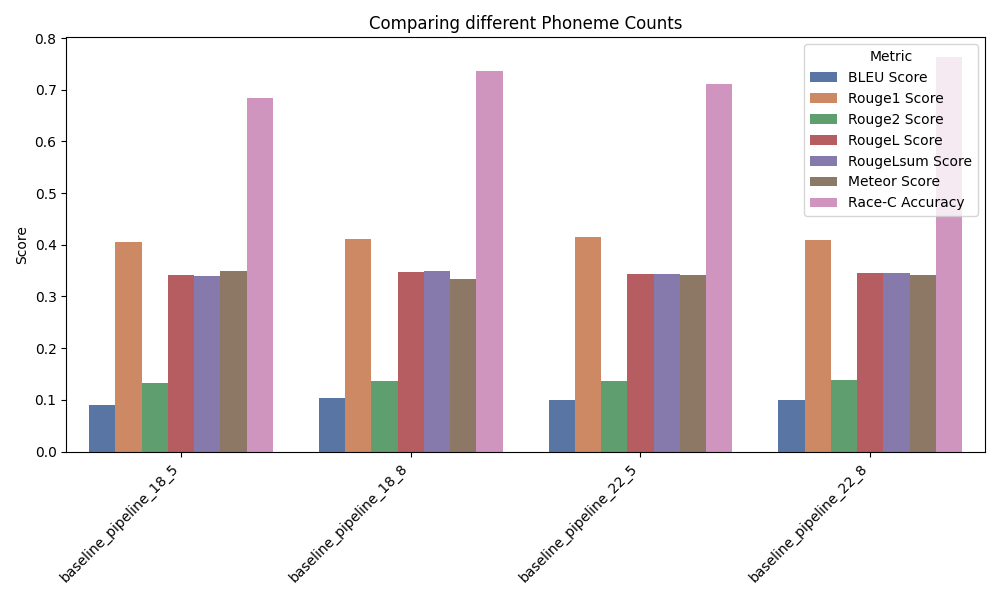
\includegraphics[width=0.7\linewidth]{figures/results/1_effect_of_phoneme_count.png}
    \caption{Comparing the Effects of different phoneme counts}
    \label{fig:compare-phoneme-count}
\end{figure}

As we can see in Figure \ref{fig:compare-phoneme-count}, the phoneme count does not seem to have a significant effect on the translation scores
or the Race-C scores. This being the case, we can conclude that we can simplify a language by reducing the phoneme count without affecting the 
ability of the language to convey meaning. 

\section{Effect of Phonotactics}

\begin{figure}[H]  
    \centering
    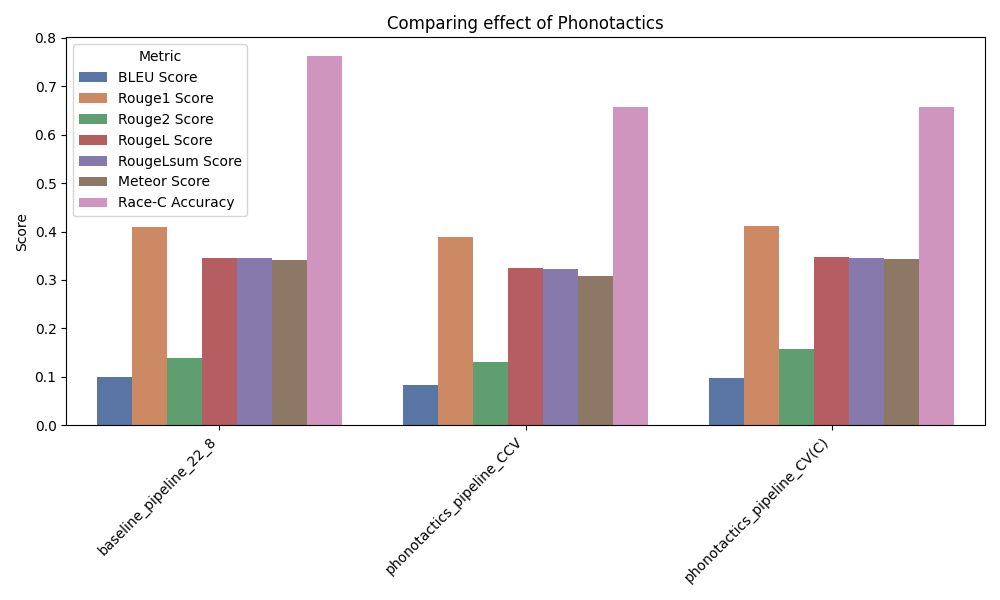
\includegraphics[width=0.7\linewidth]{figures/results/1_effect_of_phonotactics.png}
    \caption{Comparing the Effects of phonotactics}
    \label{fig:compare-phonotactics}
\end{figure}

Figure \ref{fig:compare-phonotactics} shows the effect of phonotactics on the translation scores and the Race-C scores. Again, we can see that
the phonotactics do not seem to have a significant effect either of the metrics. We can therefore conclude that we can simplify a language by 
using simplifed phonotactic rules without affecting the ability of the language to convey meaning.

\section{Effect of Grammar Rules}

\begin{figure}[H]  
    \centering
    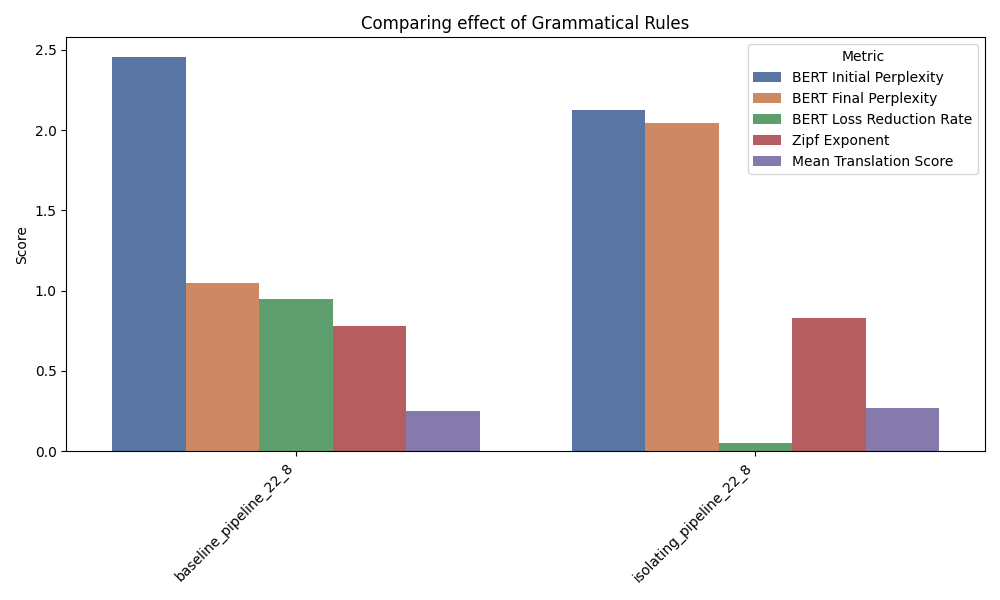
\includegraphics[width=0.7\linewidth]{figures/results/1_effect_of_grammar.png}
    \caption{Comparing different Grammatical Rules}
    \label{fig:compare-grammar}
\end{figure}

We implemented 2 different grammars, but from our results we did not find any significant difference between the Agglutinative and Isolating 
grammar modules, save for differences in the Final Perplexity in the Bert Evaluation. Further investigation is required to analyse the effects
of grammatical features in constructed languages.

\section{Effect of Vocabulary Generation method}

Figure \ref{fig:compare-vocab-gen-types} shows the effect of different simplifying vocabulary generation methods against our metrics.
We can see that both methods result in a drop in the translation scores, and in the Race-C scores. We can consider the ratio of the Mean Translation Score (MTS) and 
the Race-C Accuracy to the vocabulary size.

\begin{figure}[H]
    \centering
    \begin{subfigure}[b]{0.48\linewidth}
        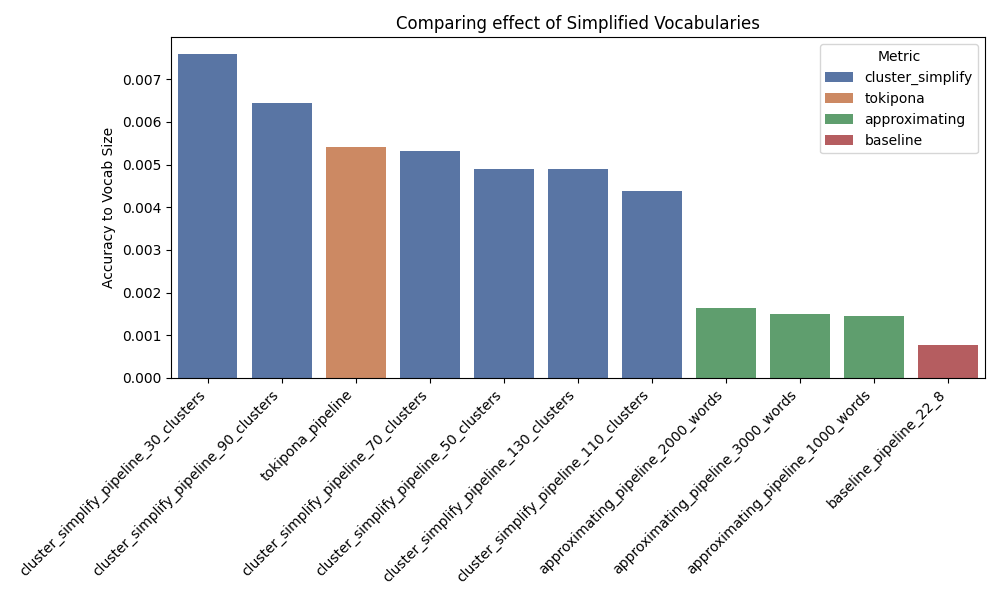
\includegraphics[width=\linewidth]{figures/results/1_effect_of_vocab_simplify.png}
        \caption{Effect of Vocabulary on Race-C Accuracy}
        \label{fig:vocabulary-effect-rc}
    \end{subfigure}
    \hfill
    \begin{subfigure}[b]{0.48\textwidth}
        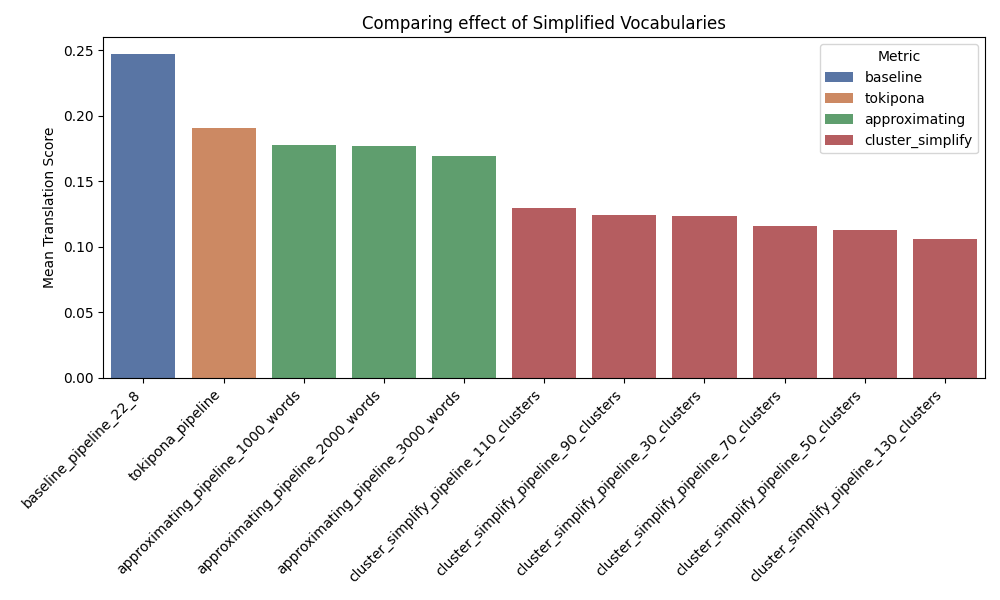
\includegraphics[width=\linewidth]{figures/results/1_effect_of_vocab_simplify_mts.png}
        \caption{Effect of Vocabulary on MTS}
        \label{fig:vocabulary-effect-mts}
    \end{subfigure}
    \caption{Effect of Simplified Vocabulary.}
    \label{fig:vocabulary-effect-mts-rc}
\end{figure}

From Figure \ref{fig:vocabulary-effect-mts}, we can see that the drop in MTS Score is much more significant, with the baseline having the highest ratio. However,
as we can see from Figure \ref{fig:vocabulary-effect-rc}, The cluster-simplify and approximating methods perform better in terms of accuracy to vocabulary size.
For all practical purposes, we can argue that the performance on the Reading Comprehension dataset is a better proxy for the performance of the language, rather than the MTS scores,
which heavily depend on n-gram similarity.

\section{Effect of Language Model Temperature}
We compared the effects of different model temperatures on the evaluations, with the same baseline pipeline. The baseline was run with a temperature value of 
\texttt{0.2}. From Figure \ref{fig:compare-temperature}, we can see that the higher model temperature seems to degrade the result of some scores, but 
does not seem to have a significant effect with a lower temperature. We can conclude that the results can be reproduced at different model temperatures, as long as 
the temperature is not too high. 
\begin{figure}[H]  
    \centering
    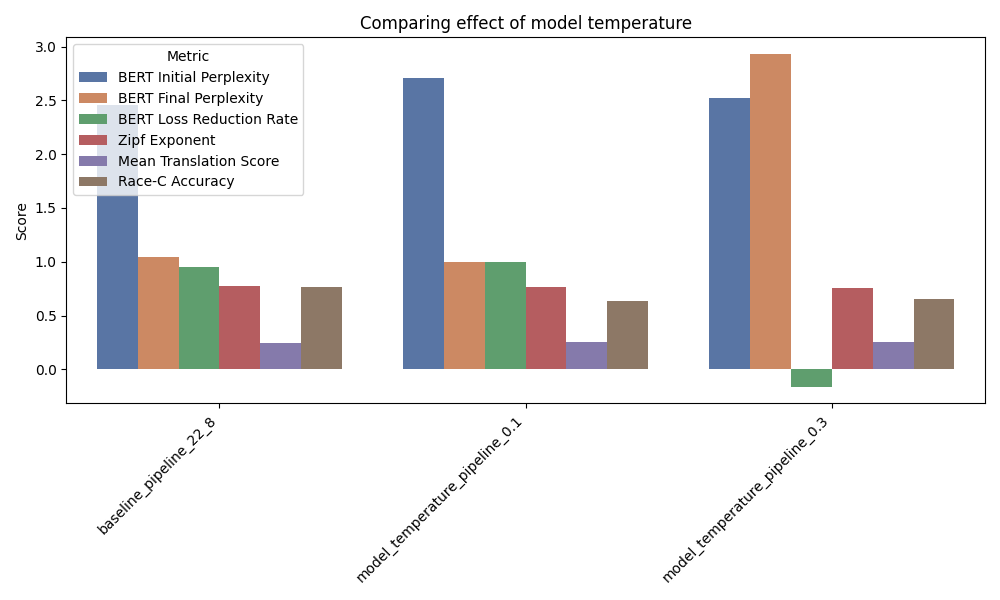
\includegraphics[width=0.7\linewidth]{figures/results/1_effect_of_model_temperature.png}
    \caption{Effect of Model Temperature}
    \label{fig:compare-temperature}
\end{figure}


\section{Conclusion}
This thesis set out to investigate whether pre-trained Large Language Models (LLMs) can aid in the systematic construction of minimal, efficient 
languages that preserve communicative utility. By developing a modular pipeline that integrates phonology, phonotactics, grammar, vocabulary, and multiple evaluation strategies, 
we were able to design and assess a variety of constructed languages (ConLangs) under different constraints.

The results demonstrate that significant simplifications are possible in multiple linguistic subsystems, such as reducing phoneme inventory and grammar complexity,
without substantially degrading performance on machine translation or comprehension tasks. In particular, reading comprehension scores remained relatively robust even in highly 
simplified setups, indicating that core meaning can be preserved despite a reduction in language complexity. Additionally, the adherence to Zipf's Law in many generated languages 
suggests that even artificial languages can naturally align with linguistic patterns found in human languages.

Our experiments show that LLMs can effectively support language generation and evaluation, acting as tools to explore the trade-off between efficiency and expressiveness in language design. 
The modularity of our framework allows for targeted ablation studies, making it a flexible foundation for future research in computational linguistics and language optimization.

In essence, this work provides strong evidence that LLMs can assist in creating interpretable, compact, and efficient constructed languages, 
opening new avenues for both linguistic theory and applied language technology.


\section{Future Work}
The results of this thesis show that it is possible to generate simplified languages that are still able to convey meaning. However, there are still many
open areas for future work. Firstly, we can explore other different language generation methods, including more or less complex grammatical rules,
or different vocabulary generation methods. In particular, further research is required in analyzing the effects of different grammatical structures.

In addition, further research is required on metrics to evaluate the generated languages. In particular, there is more to explore
in terms of simplicity measures, which are complex to define and measure.

\chapter{Author Contributions}\label{chapter:contributions}
The codebase used for this thesis was developed by me in collaboration with Sara Visconti. I setup the initial repository and abstract classes
for the modules and pipelines as well as the data classes for the language, which was then reviewed and refactored by Sara. Both of us modified
or added to these modules and classes as needed based on experiment requirements. We also implemented specfiic modules for the experiments.

\begin{enumerate}
    \item \textbf{Phonemes}: I implemented the RandomPhonemeModule, MostCommonPhonemeModule and LanguagePhonemeModule. I also implemented the BasicAlphabetModule.
    \item \textbf{Phonotactics}: I implemented the BasicPhonotacticsModule, CustomPhonotacticsModule and SyllableBuilderModule. 
    \item \textbf{Grammar}: I implemented the BasicGrammarModule, BaselineAgglutinativeGrammarModule, and BaselineIsolatingGrammarModule. These modules built on top of Sara's Implementations of grammar features.
    \item \textbf{Vocabulary}: I implemented the FixedVocabularyModule, FromSourceVocabularyModule, ClusterSimplifyVocabularyModule, ClusterTwoLevelVocabularyModule and ApproximatingVocabularyModule. I also used the Mapping modules implemented by Sara.
    \item \textbf{Conlang}: I implemented the LLM based Source Text Translation Module.
    \item \textbf{Evaluation}: I implemented the CompressionEvaluator, DetranslationEvaluator, HTML Summary Generator and RaceCEvaluator. I used Sara's Implementation of Zipfs Law Evaluator and BertEvaluator. Sara also added the various metrics to the DetranslationEvaluator.
    \item \textbf{LLMs}: I implemented the LocalLLM and OpenAI implementation of the Remote LLM.
\end{enumerate}

We jointly developed the conceptual design and methodology. Other contributions from Sara Visconti are not reported here since they are not mentioned in this work.




\appendix{}
\chapter{Appendix}\label{chapter:appendix}

\begin{figure}
    \centering
    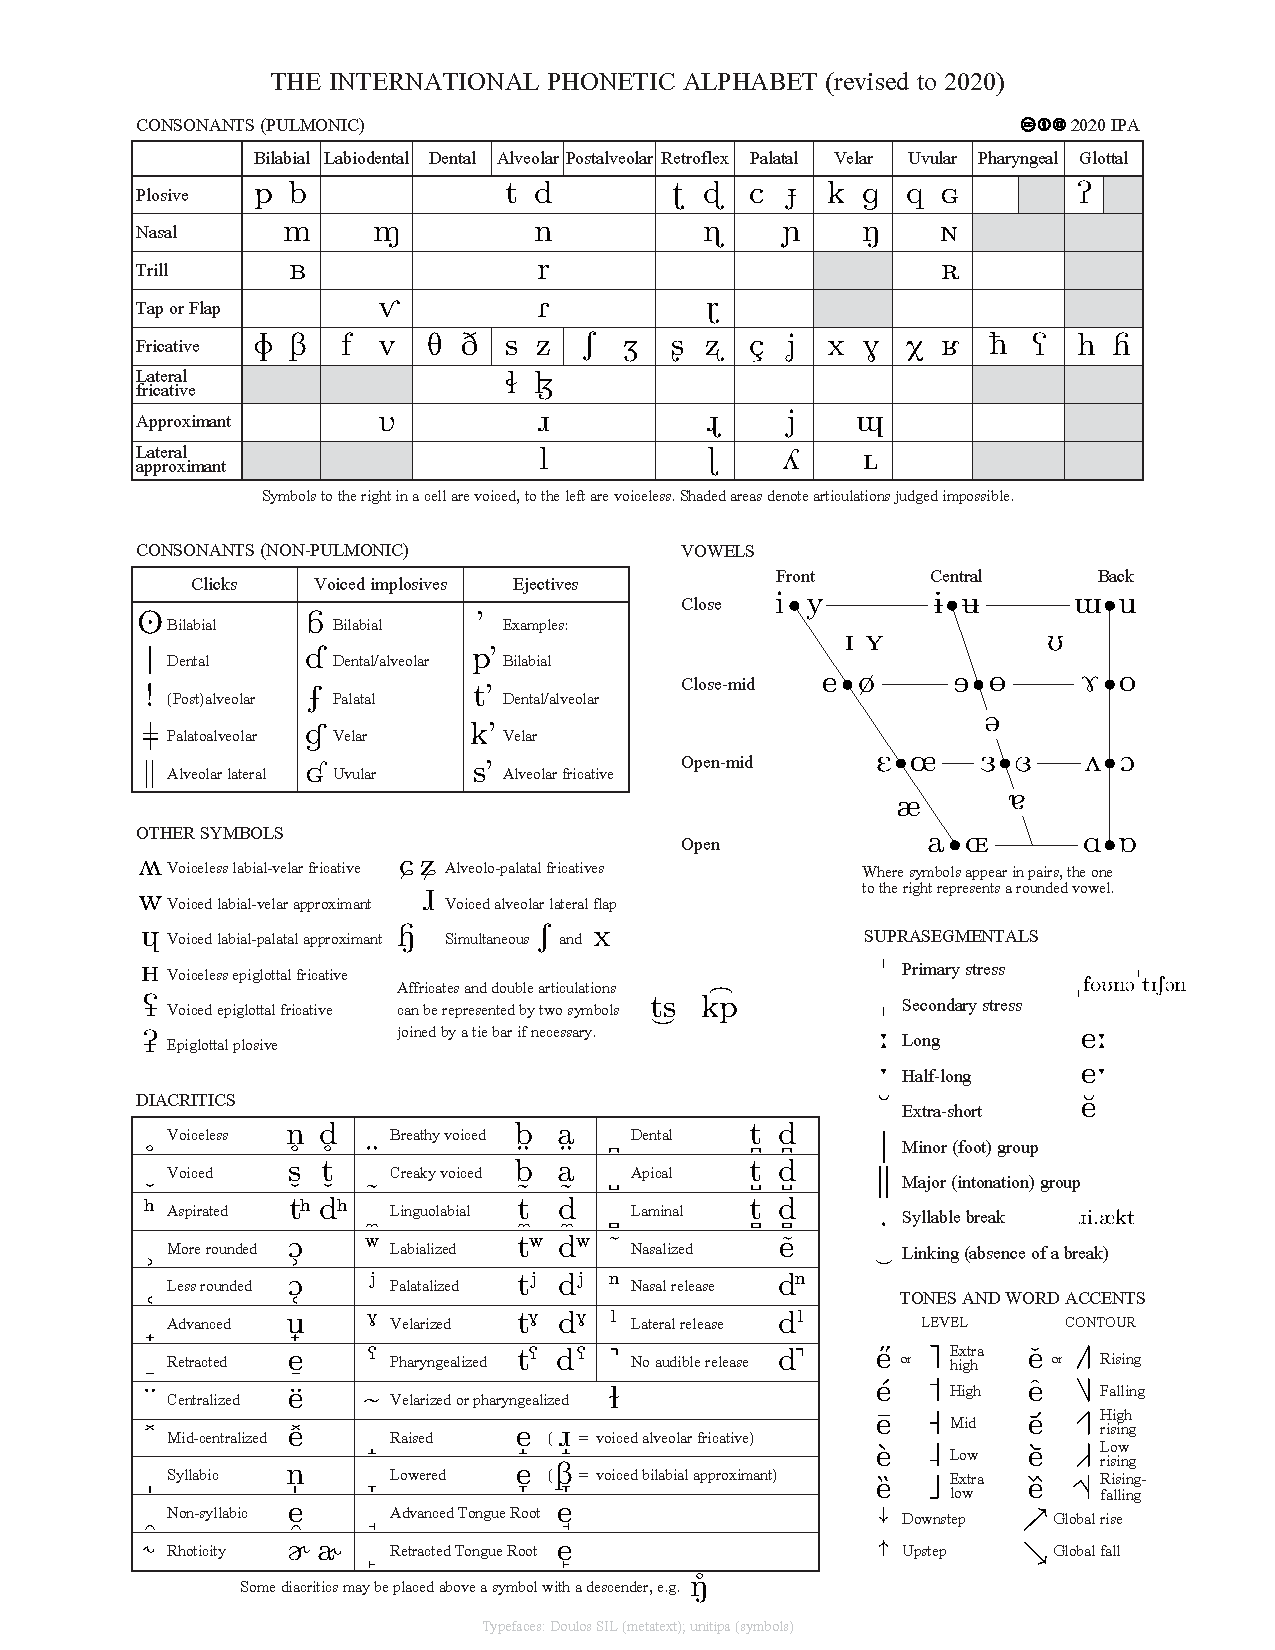
\includegraphics[width=0.9\textwidth]{figures/IPA_unitipa_2020_full.pdf}
    \caption{\href{http://www.internationalphoneticassociation.org/content/ipa-chart}{IPA Chart}, available under a Creative Commons Attribution-Sharealike 3.0 Unported License. 
    Copyright © 2018 International Phonetic Association.}
    \label{fig:ipa_chart}
\end{figure}

\microtypesetup{protrusion=false}

\addchap{Abbreviations}
\begin{acronym}
	\itemsep-.25\baselineskip
	\acro{TUM}[TUM]{Technical University of Munich}

\end{acronym}

\listoffigures{}
\listoftables{}
\microtypesetup{protrusion=true}
\printbibliography{}

\end{document}
